% ===================== CHAPITRE 2 : SOLUTION PROPOSÉE =====================

\section*{Introduction}
Ce chapitre présente les concepts clés du projet, décrit la solution proposée,
puis identifie les acteurs et les principaux cas d'utilisation.

\section{Concepts clés}
\label{sec:concepts}

\paragraph{Géolocalisation et géocodage.}
La \textbf{géolocalisation} consiste à déterminer la position d'un objet au moyen
de coordonnées géographiques (latitude, longitude) dans le système de référence
WGS~84. Le \textbf{géocodage inverse} convertit des coordonnées en une adresse
lisible~: lorsqu'un utilisateur place un marqueur sur la carte, le champ adresse
est ainsi pré-rempli automatiquement.

\paragraph{Cartographie web.}
L'affichage repose sur un fond de carte composé de \emph{tuiles} (issues
d'OpenStreetMap) sur lequel sont superposés des \emph{marqueurs}. Un mécanisme de
\emph{regroupement} (\emph{clustering}) agrège les marqueurs proches pour rester
lisible à petite échelle.

\paragraph{Découpage administratif tunisien.}
Le territoire est structuré hiérarchiquement en \textbf{gouvernorats},
subdivisés en \textbf{délégations}, elles-mêmes composées de
\textbf{secteurs / localités}. Ce découpage sert de référentiel d'adressage~:
chaque annonce est rattachée à un triplet (gouvernorat, délégation, localité) en
plus de ses coordonnées exactes.

\paragraph{Architecture client--serveur.}
La solution est pensée en trois niveaux~: un client web (navigateur), un serveur
applicatif exposant une \textbf{API} (interface de programmation) et un serveur
de \textbf{base de données}. Ce découpage guide la conception mais son
implémentation sort du périmètre de ce rapport.

\paragraph{Modélisation.}
La conception s'appuie sur \textbf{UML} pour les besoins (cas d'utilisation), la
structure (classes) et le comportement (séquence), et sur une approche de type
\textbf{Merise} pour la base de données (MCD, MLD, dictionnaire de données).

\section{Présentation de la solution}
\label{sec:solution}

La plateforme proposée est un site web responsive permettant~:
\begin{itemize}[label=\textbullet,itemsep=1pt]
  \item à un \textbf{visiteur}~: explorer les biens sur une carte interactive et
        via des filtres, consulter les fiches, comparer, contacter les
        annonceurs~;
  \item à un \textbf{particulier}~: créer un compte, publier une annonce
        géolocalisée, gérer favoris et alertes~;
  \item à une \textbf{agence} / un \textbf{promoteur}~: gérer un portefeuille
        d'annonces, des agents et un tableau de bord~;
  \item à un \textbf{administrateur}~: modérer les annonces et gérer les comptes.
\end{itemize}

\paragraph{Principes directeurs.}
\begin{itemize}[label=\textbullet,itemsep=1pt]
  \item \textbf{La carte au centre}~: la recherche cartographique est le
        parcours principal, la liste en étant une vue alternative synchronisée~;
  \item \textbf{Double adressage}~: référentiel administratif structuré
        \emph{et} coordonnées GPS, pour concilier filtrage et précision~;
  \item \textbf{Mobile-first}~: conception pensée d'abord pour le téléphone.
\end{itemize}

\begin{figure}[H]
  \centering
  \begin{tikzpicture}[
      node distance=1cm and 1.4cm,
      box/.style={draw, rounded corners, align=center, minimum width=3cm, minimum height=0.9cm, fill=codebg},
      ext/.style={draw, dashed, rounded corners, align=center, minimum width=3cm, minimum height=0.9cm}]
    \node[box] (client) {Client web\\(carte interactive)};
    \node[box, below=of client] (api) {API};
    \node[box, below=of api] (db) {Base de données};
    \node[ext, right=of api] (osm) {Fond de carte \&\\géocodage (OSM)};
    \draw[->] (client) -- (api);
    \draw[->] (api) -- (db);
    \draw[->, dashed] (client) -- (osm);
  \end{tikzpicture}
  \caption{Architecture fonctionnelle (vue de conception)}
  \label{fig:archi-fonctionnelle}
\end{figure}

\section{Spécification des besoins}
\label{sec:specification}

\subsection{Acteurs}

\begin{table}[H]
\centering
\renewcommand{\arraystretch}{1.25}
\begin{tabularx}{\linewidth}{>{\bfseries}p{3cm} X}
\toprule
Acteur & Rôle vis-à-vis du système \\
\midrule
Visiteur       & Non authentifié~: consulte et recherche les biens. \\
Particulier    & Publie et gère ses annonces, favoris et alertes. \\
Agent          & Publie des annonces pour le compte d'une agence. \\
Agence / Promoteur & Gèrent un portefeuille d'annonces, des agents, un tableau de bord. \\
Administrateur & Modère les annonces, gère comptes et référentiels. \\
Services externes & Fond de carte et géocodage (OpenStreetMap). \\
\bottomrule
\end{tabularx}
\caption{Acteurs du système}
\label{tab:acteurs}
\end{table}

\subsection{Diagramme de cas d'utilisation global}
\begin{figure}[H]
  \centering
  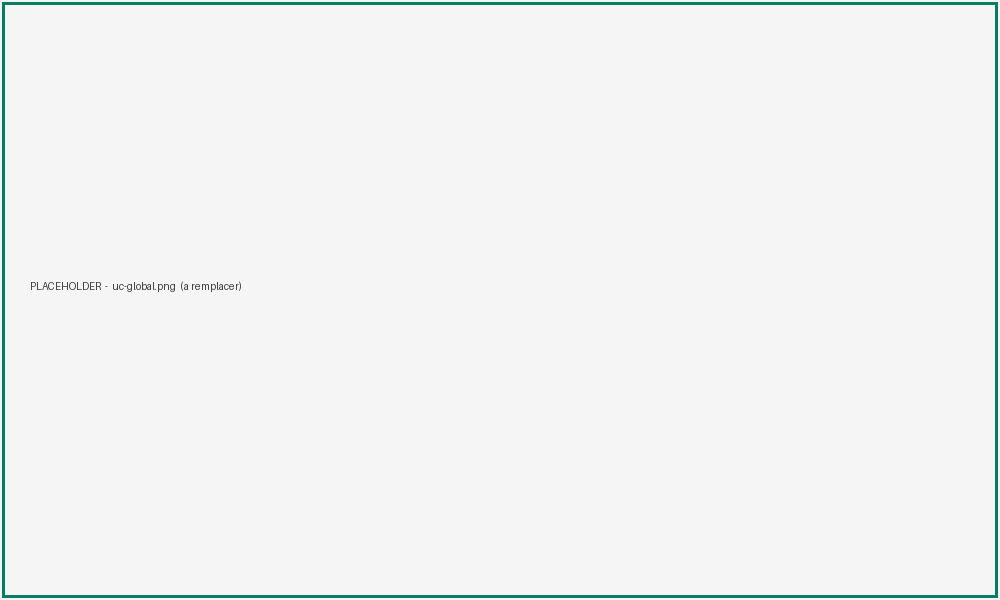
\includegraphics[width=0.9\linewidth]{images/uc-global.png} % À FOURNIR
  \caption{Diagramme de cas d'utilisation global}
  \label{fig:uc-global}
\end{figure}

\subsection{Description des cas d'utilisation principaux}

\paragraph{CU-01 : Rechercher un bien sur la carte.}
\begin{table}[H]
\centering
\renewcommand{\arraystretch}{1.2}
\begin{tabularx}{\linewidth}{>{\bfseries}p{2.8cm} X}
\toprule
Acteur         & Visiteur \\
Pré-condition  & La page de recherche cartographique est ouverte. \\
Scénario nominal &
1.~L'acteur déplace / zoome la carte.\newline
2.~Le système renvoie les biens situés dans l'emprise visible.\newline
3.~Les marqueurs sont affichés (regroupés si nombreux).\newline
4.~L'acteur clique un marqueur, consulte l'aperçu, puis ouvre la fiche. \\
Alternative    & 2a.~Aucun bien dans l'emprise~: message « aucun résultat ». \\
Post-condition & Liste et carte synchronisées sur la zone visible. \\
\bottomrule
\end{tabularx}
\caption{CU-01 « Rechercher un bien sur la carte »}
\label{tab:cu-recherche-carte}
\end{table}

\paragraph{CU-02 : Publier une annonce géolocalisée.}
\begin{table}[H]
\centering
\renewcommand{\arraystretch}{1.2}
\begin{tabularx}{\linewidth}{>{\bfseries}p{2.8cm} X}
\toprule
Acteur         & Particulier (ou Agent) \\
Pré-condition  & L'acteur est authentifié. \\
Scénario nominal &
1.~Saisie des caractéristiques du bien (type, prix, surface\ldots).\newline
2.~Choix du gouvernorat, de la délégation et de la localité.\newline
3.~Placement d'un marqueur sur la carte~; géocodage inverse et pré-remplissage
de l'adresse.\newline
4.~Ajout et réordonnancement des photos.\newline
5.~Soumission~; l'annonce passe à l'état « en attente ». \\
Alternative    & 5a.~Champs obligatoires manquants~: signalement des erreurs. \\
Post-condition & Une annonce en attente de modération est créée. \\
\bottomrule
\end{tabularx}
\caption{CU-02 « Publier une annonce géolocalisée »}
\label{tab:cu-publier}
\end{table}

\paragraph{CU-03 : Modérer une annonce.}
\begin{table}[H]
\centering
\renewcommand{\arraystretch}{1.2}
\begin{tabularx}{\linewidth}{>{\bfseries}p{2.8cm} X}
\toprule
Acteur         & Administrateur \\
Pré-condition  & Au moins une annonce est « en attente ». \\
Scénario nominal &
1.~Consultation de la file de modération.\newline
2.~Vérification du contenu, des photos et de la localisation.\newline
3.~Approbation~: l'annonce devient publique. \\
Alternative    & 3a.~Refus avec un ou plusieurs motifs et un message~; l'auteur
est notifié. \\
Post-condition & État de l'annonce~: « approuvée » ou « refusée ». \\
\bottomrule
\end{tabularx}
\caption{CU-03 « Modérer une annonce »}
\label{tab:cu-moderer}
\end{table}

\section*{Conclusion}
Les concepts clés, la solution et la spécification des besoins sont posés. Le
chapitre suivant traduit ces besoins en conception détaillée.
